% Options here are passed to the article class.
% Most common options: 10pt, 11pt, 12pt
\documentclass[10pt]{datasheet}

% Input encoding and typographical rules for English language
\usepackage[utf8]{inputenc}
\usepackage[english]{babel}
\usepackage[english]{isodate}

% tikz is used to draw images in this example, but you can
% also use \includegraphics{}.
\usepackage{graphicx}
\usepackage{float}
\usepackage{subcaption}

% These define global texts that are used in headers and titles.
\title{EB01: Minewave Fixed Bulk Slice}
\author{Basil}
\tags{external-bulk, fixed-bulk, multi-slice}
\date{25 December 2024}
\revision{Revision 1}
\begin{document}
\maketitle

\section{Features}

\begin{itemize}
\item{1.1 million item capacity}
\item{Multi-slicing compatible}
\item{Input overflow protection}
\item{Fully hopperlocked}
\end{itemize}

\section{Applications}

\begin{itemize}
\item{External bulk storage}
\end{itemize}

\section{General Description}
The EB01 Minewave Fixed Bulk Slice is a device that can be stacked to create a fixed external bulk storage system. The device interfaces with an decoder (not included) and a controller (not included) to automatically store and retrieve items with redstone control. Multi-slicing, the ability to set multiple slices to the same code, is supported. These multi-sliced slices need not be adjacent.

\vfill\break

\begin{figure}[H]
    \centering
    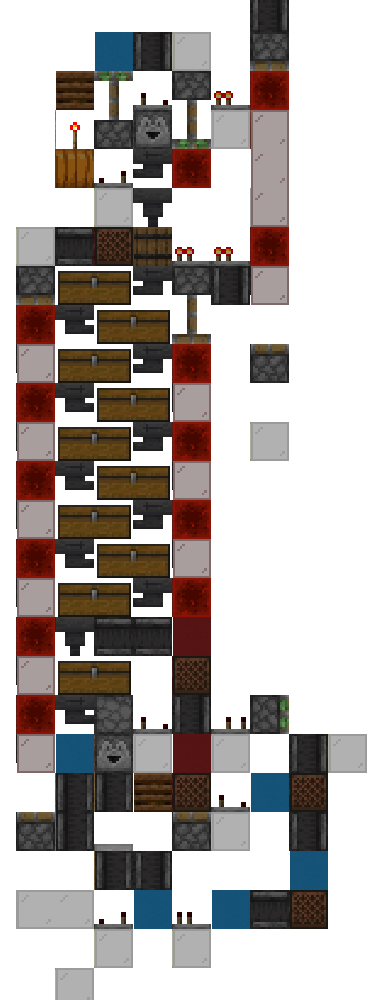
\includegraphics[width=0.3\textwidth]{area_render_15_.png}
    \caption{\centering Minewave Fixed Bulk Slice}
\end{figure}

% For wide tables, a single column layout is better. It can be switched
% page-by-page.
\onecolumn
\section{Connecting the output triggers}
The output triggers are connected to the controller from the back of the bulk to preserve the correct update order for the dropperline. The output trigger lines must be connected with the following timings: 0gt - output trigger 1, 4gt - output trigger 2, 10gt - output trigger 3.

\begin{figure}[H]
    \centering
    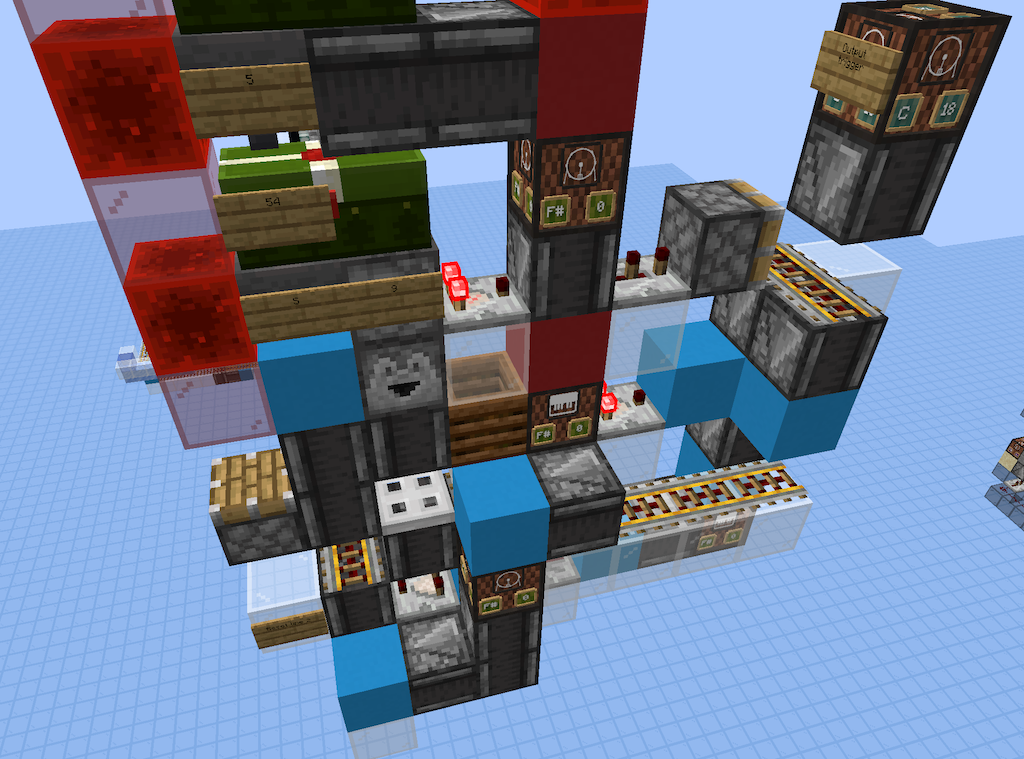
\includegraphics[width=0.6\textwidth]{trigger.png}
    \caption{\centering Output Trigger Wiring}
\end{figure}

\section{Rail extensions}
Rail extensions, necessary in order to expand the bulk storage beyond nine slices, must be aligned in the following manner.

\begin{figure}[H]
    \centering
    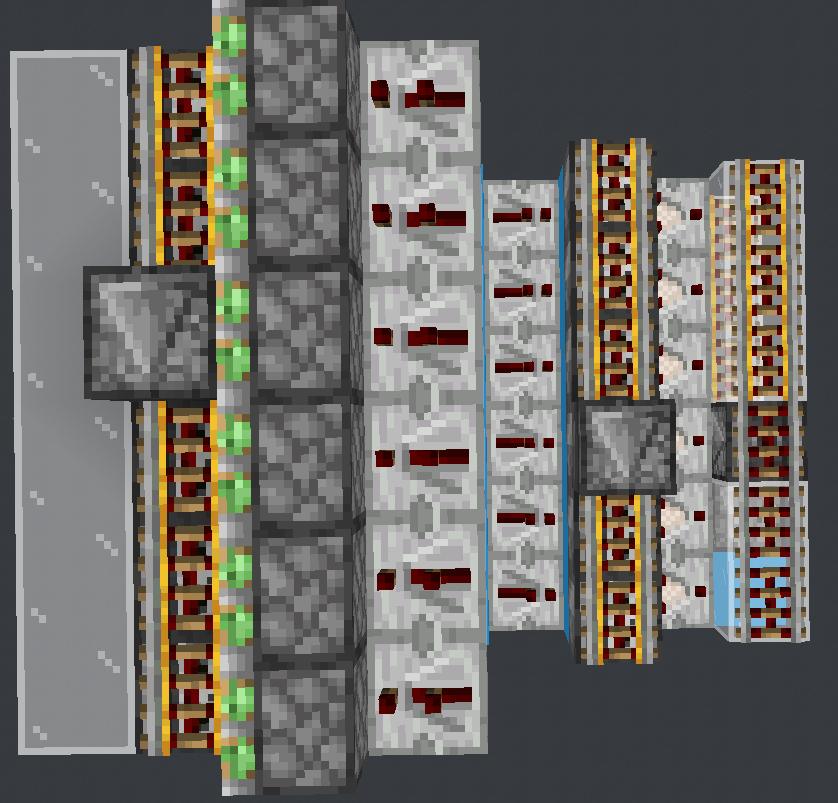
\includegraphics[width=0.4\textwidth]{ext1.png}
    \caption{\centering Rail Extension Alignment}
\end{figure}

\begin{figure}[H]
    \centering
    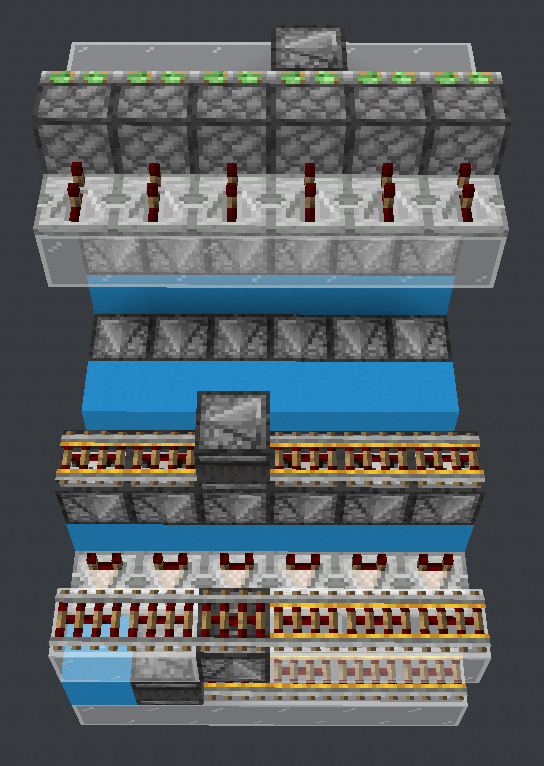
\includegraphics[width=0.4\textwidth]{ext2.png}
    \caption{\centering Rail Extension Alignment, Side View}
\end{figure}

\newpage
\section{Device Specifications}

\begin{table}[H]
    \caption{Inputs}
    \begin{tabularx}{\textwidth}{l | c | X}
        \thickhline
        \textbf{Name} & \textbf{Range} & \textbf{Description} \\
        \hline
        Box input & Box & Dropperline input for transporting boxes to the slices. \\
        \hline
        Slice activation & Pulse & Activates the slice to store or retrieve boxes. Connect to a decoder. Piston input. \\
        \hline
        Output trigger 1 & Pulse & Selects the slice for output. \\
        \hline
        Output trigger 2 & Pulse & Triggers the output of the slice. Should be pulsed 4gt after output trigger 1. \\
        \hline
        Output trigger 3 & Pulse & Triggers the output dropperline. Should be pulsed 10gt after output trigger 1. \\
        \hline
        Reset lines 1 \& 2 & Pulse & Disables the slice. \\
        \thickhline
\end{tabularx}
\end{table}

\begin{table}[H]
    \caption{Outputs}
    \begin{tabularx}{\textwidth}{l | c | X}
        \thickhline
        \textbf{Name} & \textbf{Range} & \textbf{Description} \\
        \hline
        Box output & Box & Dropperline output for transporting boxes from the slices. \\
        \thickhline
\end{tabularx}
\end{table}

\begin{table}[H]
    \caption{Device Specifications}
    \begin{tabularx}{\textwidth}{l | c c c | c | X}
        \thickhline
        \textbf{Parameter} & \textbf{Min.} & \textbf{Typ.} & \textbf{Max.} &
        \textbf{Unit} & \textbf{Conditions} \\
        \hline
        Throughput  & 8 & - & - & gt & Input/output throughput \\
        \hline
        Latency    & 18 & - & - & gt & From output trigger to dropper activation. \\
        \hline
        MC Version & 1.16 & 1.21.4 & - & MCV & Latest version at time of writing: 1.21.4\\
        \hline
        Dimensions & & 1 x 26 x 29 & & Blocks & \\
        \thickhline
\end{tabularx}
\end{table}

\section{Testing Data}
\begin{table}[H]
\caption{Executed Tests}
\begin{tabularx}{\textwidth}{l | X}
    \thickhline
    \textbf{Test} & \textbf{Result} \\
    \hline
    Output test & Device was able to output boxes correctly using the output triggers. \\
    \thickhline
\end{tabularx}
\end{table}

\section{Download Information}
\begin{table}[h]
    \caption{Download Information}
    \begin{tabularx}{\textwidth}{l | l | l | X}
        \thickhline
        \textbf{Identifier} & \textbf{MC} & \textbf{File} & \textbf{Description} \\
        \hline
        EB01 & 1.21.4 & \href{https://github.com/Soontech-Annals/Archive/blob/8413f90a054b6c415703bae02badeba7541344f6/Archive/external-bulk/EB01\%20Minewave\%20Fixed\%20Bulk\%20Slice/EB01\_Minewave\_Fixed\_Bulk\_Slice.litematic?raw=1}{EB01\_Minewave\_Fixed\_Bulk\_Slice.litematic} & Schematic of device. \\
        \hline
        \thickhline
    \end{tabularx}
\end{table}

\end{document}

